\documentclass[11pt]{article}

\usepackage[UTF8]{ctex} % for Chinese 
% \setCJKmainfont[ItalicFont=Noto Sans CJK SC Bold, BoldFont=Noto Serif CJK SC Black]{Noto Serif CJK SC} % for Chinese

% \setCJKmainfont{Noto Serif CJK SC} % for Chinese

\usepackage{setspace}
\usepackage[colorlinks,linkcolor=blue,anchorcolor=red,citecolor=black]{hyperref}
\usepackage{lineno}
\usepackage{booktabs}
\usepackage{graphicx}
\usepackage{float}
\usepackage{floatrow}
\usepackage{subfigure}
\usepackage{caption}
\usepackage{subcaption}
\usepackage{geometry}
\usepackage{multirow}
\usepackage{longtable}
\usepackage{lscape}
\usepackage{booktabs}
\usepackage{natbib}
\usepackage{natbibspacing}
\usepackage[toc,page]{appendix}
\usepackage{makecell}

\title{墨子}
\date{}

\linespread{1.5}
\geometry{left=2cm,right=2cm,top=2cm,bottom=2cm}

\begin{document}

  \maketitle
  
  \begin{figure}
    \centering
    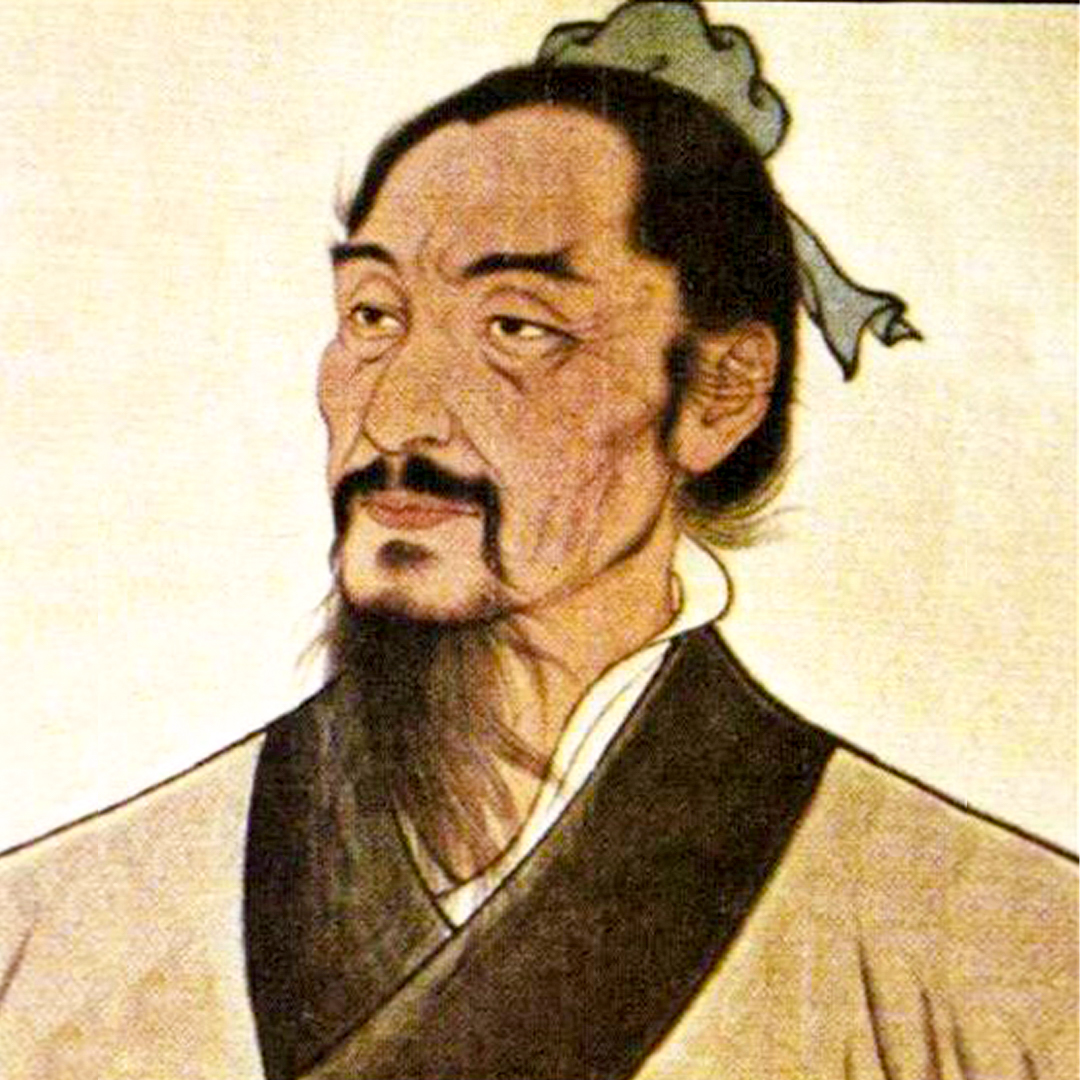
\includegraphics[width=0.8\textwidth]{../Figures/MoZi.jpg}
    \caption{墨子像。}
  \end{figure}
  \newpage

  \linenumbers

墨子名翟,相传为宋大夫,生平不可考。
其时代大抵在孔子之后,孟子之前。
其学于战国大盛,孟、庄、荀、韩诸子皆称其为显学。
然自秦燹后,墨学大衰。

\newline

考墨子之学,其着力点在于如何“兴天下之利”。
此一“利”字纯就物质方面着眼,故功利主义为墨学之一精神主脉。
此外,对于社会秩序之建立,墨子持权威主义态度。
此为墨学之另一精神主脉。

\section{兼爱}
“兼爱”指普遍相爱。
换言之,所有人都应该不分高低贵贱,彼此相爱。
墨子之博爱精神,其出发点不在于道德,而是着眼于平乱这一现实问题。
墨子认为,社会混乱之根源在于不兼爱。
由于不兼爱,故有亏人自利之行径,冲突由此而来,遂生乱矣。
此理不仅针对人与人之间的矛盾侵害,家族与家族、国家与国家之间亦是如此。
《墨子·兼爱上》载:

\textit{圣人以治天下为事者也,不可不察乱之所自起。当察乱何自起?起不相爱。臣子之不孝君父,所谓乱也。子自爱不爱父,故亏父而自利;弟自爱不爱兄,故亏兄而自利;臣自爱不爱君,故亏君而自利,此所谓乱也。虽父之不慈子,兄之不慈弟,君之不慈臣,此亦天下之所谓乱也。父自爱也不爱子,故亏子而自利;兄自爱也不爱弟,故亏弟而自利;君自爱也不爱臣,故亏臣而自利。是何也?皆起不相爱。虽至天下之为盗贼者亦然,盗爱其室不爱其异室,故窃异室以利其室;贼爱其身不爱人,故贼人以利其身。此何也?皆起不相爱。虽至大夫之相乱家,诸侯之相攻国者亦然。大夫各爱其家,不爱异家,故乱异家以利其家;诸侯各爱其国,不爱异国,故攻异国以利其国,天下之乱物具此而已矣。察此何自起?皆起不相爱。}

由此,欲平乱,则需推行兼爱。
《墨子·兼爱上》载:

\textit{若使天下兼相爱,爱人若爱其身,犹有不孝者乎?视父兄与君若其身,恶施不孝?犹有不慈者乎?视弟、子与臣若其身,恶施不慈?故不孝不慈亡有,犹有盗贼乎?故视人之室若其室,谁窃?视人身若其身,谁贼?故盗贼亡有。犹有大夫之相乱家、诸侯之相攻国者乎?视人家若其家,谁乱?视人国若其国,谁攻?故大夫之相乱家,诸侯之相攻国者亡有。若使天下兼相爱,国与国不相攻,家与家不相乱,盗贼无有,君臣父子皆能孝慈,若此,则天下治。}

更进一步,墨子强调兼爱为必可行、不难行、必有效之主张。
《墨子·兼爱中》载:

\textit{子墨子言曰:“天下之士君子,特不识其利、辩其故也。今若夫攻城野战,杀身为名,此天下百姓之所皆难也。若君说之,则士众能为之。况于兼相爱、交相利,则与此异。夫爱人者,人必从而爱之;利人者,人必从而利之;恶人者,人必从而恶之;害人者,人必从而害之。此何难之有?特上弗以为政、士不以为行故也。”昔者晋文公好士之恶衣,故文公之臣,皆牂羊之裘,韦以带剑,练帛之冠,入以见于君,出以践于朝。是其故何也?君说之,故臣为之也。昔者楚灵王好士细要,故灵王之臣,皆以一饭为节,胁息然后带,扶墙然后起。比期年,朝有黧黑之色。是其故何也?君说之,故臣能之也。昔越王句践好士之勇,教驯其臣,和合之,焚舟失火,试其士曰:“越国之宝尽在此!”越王亲自鼓其士而进之,士闻鼓音,破碎乱行,蹈火而死者,左右百人有余,越王击金而退之。是故子墨子言曰:“乃若夫少食、恶衣、杀人而为名,此天下百姓之所皆难也。若苟君说之,则众能为之;况兼相爱、交相利,与此异矣!夫爱人者,人亦从而爱之;利人者,人亦从而利之;恶人者,人亦从而恶之;害人者,人亦从 而害之。此何难之有焉?特士不以为政而士不以为行故也。}

\newline

需要注意的是,墨子以不兼爱为乱之根源,虽于理可通,但其理论单薄。
试想,人若不相爱,可能起冲突而有亏人自利之行为,亦可能彼此划清界限,井水不犯河水。
若深究乱之根源,可论客观条件之影响,如人与人需争夺有限之资源而起冲突;亦可论主观因素之影响,如将亏人自利归因于人性之贪婪,就自觉心一方面展开论述。
然而此类延伸不见于墨子之学。
盖墨子论兼爱,其着重点在于兼爱可达平乱之功效。
倘人人均能爱人如爱己,则自不会损人利己,乱自平矣。
此为兼爱理论之核心,余者皆为末节。
由此,墨学之功利主义态度已然显现。

\section{天志}
墨子主张兼爱,虽强调其实际效用,但亦需论其正当性,肯定兼爱之价值。
理论上说,墨子既以兼爱为平乱之有效手段,则只需论平乱之价值便可证立兼爱之价值。
而欲证平乱之价值,直言乱之危害便可。
由此,兼爱便有作为工具之价值。
此一论证思路于非攻理论中有所暗示,但非墨子证立兼爱价值之主要途径。

\newline

墨子论兼爱之价值,将其归于“天志”。
天志欲人兼爱,故兼爱有价值;天志不欲乱,故平乱有价值。
《墨子·天志上》载:

\textit{顺天意者,兼相爱,交相利,必得赏;反天意者,别相恶,交相贼,必得罚。}

《天志中》又谓:

\textit{天之意不欲大国之攻小国也,大家之乱小家也。}

\newline

更进一步,天志为超越性主宰。
其所欲者即为正当,即有价值;其所不欲者即为不正当。
故人必为天志之所欲,戒天志之所恶。
天志作为最高权威尺度,其根据在于“天为贵,天知”。
《墨子·天志中》载:

\textit{子墨子言曰:“今天下之君子之欲为仁义者,则不可不察义之所从出。既曰不可以不察义之所从出,然则义何从出?”子墨子曰:“义不从愚且贱者出,必自贵且知者出。何以知义之不从愚且贱者出,而必自贵且知者出也?曰:义者,善政也。何以知义之为善政也?曰:天下有义则治,无义则乱,是以知义之为善政也。夫愚且贱者,不得为政乎贵且知者,然后得为政乎愚且贱者,此吾所以知义之不从愚且贱者出,而必自贵且知者出也。然则孰为贵?孰为知?曰:天为贵,天为知而已矣。然则义果自天出矣。”}

\newline

更进一步,墨子又将天志与天子相关联,言天志正天子,而天子正天下。
《墨子·天志下》云:
\textit{是故庶人不得次己而为正,有士正之;士不得次己而为正,有大夫正之;大夫不得次己而为正,有诸侯正之;诸俟不得次己而为正,有三公正之;三公不得次己而为正,有天子正之;天子不得次己而为正,有天正之。今天下之士君子,皆明于天子之正天下也,而不明于天之正天子也。是故古者圣人明以此说人,曰:“天子有善,天能赏之;天子有过,天能罚之。”}

由此,作为超越主宰之天志与人间政治主宰相关联,遂产生基于权威主义的国家理论,即尚同。
。
\section{尚同}
尚同,即在下者需服从在上者。
此说之主旨在于构建一上通天志、下达万民之权威体系。
为说明在下者必须同乎上,墨子提出一权威主义国家起源理论。
《墨子·尚同上》谓:

\textit{古者民始生,未有刑政之时,盖其语,人异义。是以一人则一义,二人则二义,十人则十义。其人兹众,其所谓义者亦兹众。是以人是其义,以非人之义,故交相非也。是以内者父子兄弟作,离散不能相和合;天下之百姓,皆以水火毒药相亏害。至有余力,不能以相劳;腐朽余财,不以相分;隐匿良道,不以相教。天下之乱,若禽兽然。夫明乎天下之所以乱者,生于无政长。是故选天下之贤可者,立以为天子。天子立,以其力为未足,又选天下之贤可者,置立之以为三公。天子、三公既以立,以天下为博大,远国异土之民,是非利害之辩,不可一二而明知,故画分万国,立诸侯国君。诸侯国君既已立,以其力为未足,又选择其国之贤可者,置立之以为正长。正长既已具,天子发政于天下之百姓,言曰:“闻善而不善,皆以告其上。上之所是,必皆是之,所非,必皆非之。上有过则规谏之,下有善则傍荐之。上同而不下比者,此上之所赏而下之所誉也。意若闻善而不善,不以告其上;上之所是弗能是,上之所非弗能非;上有过弗规谏,下有善弗傍荐;下比不能上同者,此上之所罚而百姓所毁也。”上以此为赏罚,甚明察以审信。}

墨子论国家起源,以义为出发点。
未有政府时,人各执己意,互相冲突。
欲平息此种相对主义式的混乱,遂拥立贤者为天子,自上而下构建政府机关,其根本目的在于建立一共同的价值标准以平乱。
由此,在下者必须服从在上者之统一领导,是其所是,非其所非。
如此则乱平而天下治。

\newline

至此,人人放弃自身之是非标准,而服从在上者之标准,层层上升,乃至天子。
而天子服从于天志这一超越主宰。
而天志欲人兼爱,故人人兼相爱。
天志、尚同、兼爱之说由此相关联,其权威主义立场和宗教色彩甚为明显。

\section{非攻}
非攻,即反对战争。
墨子反对征伐,主要从战争之不义和无利两个方面展开论证。
此主张可视为对作为平乱工具的兼爱之价值的论证,但注重于国与国之间的冲突,且显现墨子学说之功利主义成分。

\newline

《墨子·非攻上》论战争之不义,以其为亏人自利之极:

\textit{今有一人,入人园圃,窃其桃李,众闻则非之,上为政者,得则罚之,此何也?以亏人自利也。至攘人犬豕鸡豚,其不义又甚入人园圃窃桃李。是何故也?以亏人愈多,其不仁兹甚,罪益厚。至入人栏厩,取人马牛者,其不仁义,又甚攘人犬豕鸡豚,此何故也?以其亏人愈多。苟亏人愈多,其不仁兹甚,罪益厚。至杀不辜人也,拖其衣裘,取戈剑者,其不义,又甚入人栏厩取人马牛。此何故也?以其亏人愈多。苟亏人愈多,其不仁兹甚矣,罪益厚。当此,天下之君子皆知而非之,谓之不义。今至大为攻国,则弗知非,从而誉之,谓之义。此可谓知义与不义之别乎?
\newline
杀一人,谓之不义,必有一死罪矣。若以此说往,杀十人,十重不义,必有十死罪矣;杀百人,百重不义,必有百死罪矣。当此,天下之君子皆知而非之,谓之不义。今至大为不义攻国,则弗知非,从而誉之,谓之义,情不知其不义也,故书其言以遗后世。若知其不义也,夫奚说书其不义以遗后世哉? 今有人于此,小见黑曰黑,多见黑曰白,则必以此人为不知白黑之辩矣;少尝苦曰苦,多尝苦曰甘,则必以此人为不知甘苦之辩矣。今小为非,则知而非之;大为非攻国,则不知非,从而誉之,谓之义。此可谓知义与不义之辩乎?是以知天下之君子也,辩义与不义之乱也。}

此章抨击攻国亏人最甚,为大不义,且行文犀利,颇值一观。

\newline

攻伐不惟不义 亦无利。
《墨子·非攻中》云:

\textit{今师徒唯毋兴起,冬行恐寒,夏行恐暑,此不可以冬夏为者也。春则废民耕稼树艺,秋则废民获敛。今唯毋废一时,则百姓饥寒冻馁而死者,不可胜数。今尝计军上:竹箭、羽旄、幄幕、甲盾、拨劫,往而靡弊腑冷不反者,不可胜数。又与矛、戟、戈、剑、乘车,其列住碎拆靡弊而不反者,不可胜数。与其牛马,肥而往,瘠而反,往死亡而不反者,不可胜数。与其涂道之修远,粮食辍绝而不继,百姓死者,不可胜数也。与其居处之不安,食饭之不时,肌饱之不节,百姓之道疾病而死者,不可胜数。丧师多不可胜数,丧师尽不可胜计,则是鬼神之丧其主后,亦不可胜数。
\newline
国家发政,夺民之用,废民之利,若此甚众,然而何为为之?曰:“我贪伐胜之名,及得之利,故为之。”子墨子言曰:“计其所自胜,无所可用也;计其所得,反不如所丧者之多。”今攻三里之城,七里之郭,攻此不用锐,且无杀,而徒得此然也?杀人多必数于万,寡必数于千,然后三里之城,七里之郭且可得也。今万乘之国,虚数于千,不胜而入;广衍数于万,不胜而辟。然则土地者,所有余也;王民者,所不足也。今尽王民之死,严下上之患,以争虚城,则是弃所不足,而重所有余也。为政若此,非国之务者也。
\newline
饰攻战者言曰:“南则荆、吴之王,北则齐、晋之君,始封于天下之时,其土地之方,未至有数百里也;人徒之众,未至有数十万人也。以攻战之故,土地之博,至有数千里也;人徒之众,至有数百万人。故当攻战而不可为也。”子墨子言曰:“虽四五国则得利焉,犹谓之非行道也。譬若医之药人之有病者然,今有医于此,和合其祝药之于天下之有病者而药之。万人食此,若医四五人得利焉,犹谓之非行药也。故孝子不以食其亲,忠臣不以食其君。古者封国于天下,尚者以耳之所闻,近者以目之所见,以攻战亡者,不可胜数。”何以知其然也?东方有莒之国者,其为国甚小,闲于大国之闲,不敬事于大,大国亦弗之从而爱利,是以东者越人夹削其壤地,西者齐人兼而有之。计莒之所以亡于齐、越之间者,以是攻战也。虽南者陈、蔡,其所以亡于吴、越之间者,亦以攻战。虽北者且不一著何,其所以亡于燕代、胡貊之闲者,亦以攻战也。是故子墨子言曰:“古者王公大人,情欲得而恶失,欲安而恶危,故当攻战,而不可不非。”}

墨子谓兴兵征伐耗资巨大而所得甚微,乃得不偿失之举。纵然征战或可使国家强大,一如荆吴之王,齐晋之君,但所或利者仅为一两国,所兴者非天下之利,亦是无利。况且因好战而亡者不可胜数,足见攻战之非。

总而言之,墨子非攻,自其不义和无利两方面论述。
于理论脉络,则非攻可由兼爱推出,亦可反证兼爱之工具价值。
盖人应遵天志,兼相爱,交相利,自不可起战争。
兼爱可止战,使人免于战争之危害,故兼爱有作为工具之价值。

\section{非儒}
战国之时,儒墨并称显学,并互相为敌。
盖墨子之功利主义和权威主义哲学,本与儒家之德性理论不相容。
儒墨皆言“爱人”,但儒者之“仁者爱人”,系自觉心之本有。
墨子之兼爱,系由外部附加于人。
墨子谓人之所以需要兼爱,其原因在于超越主宰和政府权威之命令以及“兴天下之利”的需求。
儒者批驳墨子之言论,由于资料有限,难以作一专题讨论。
而今传《墨子》中,不乏批判儒者之论。
此类论述,虽鲜有触及儒学贵德性之根本者,但其中所透露出的功利主义立场甚明,可作为墨子理论之补充。

\newline

墨子非儒,首讥讽儒者不事生产,且所倡导之礼乐虚伪无用,劳民伤财。
其中又尤其以音乐为无用。
此类文化艺术无本有价值,作为工具亦“不中万民之利”,故应当禁止。
由此可见墨子之功利主义态度。
后世荀子评之曰:“墨子蔽于用而不知文”,即针对此论。

\newline

其次,墨子批判儒者“法古”。
谓一切事物皆有其创作者。
今日所法之古,于前朝乃是一新。
若以法古之教条反对革新,则古人之新创皆为不当,焉能法之。
此论看似有据,实不得儒者论周礼之要旨。
儒学将外在的社会秩序归因于人之自觉,树确立人之主宰地位。
则人之自觉所追求之社会秩序,其具体内容究竟为何?
答曰:周礼。
故儒者贵礼重乐,实与法古无关。

\newline

最后,墨子讥嘲孔子之诈伪,言其喜弄阴谋。
然所言事迹于史难考且无理论意义,兹不赘述。

\end{document}